%!TEX root = main.tex
\section{Perspective Resolution in Crowdsourced Image Segmentation}
\subsection{Worker Clustering}
Our clustering-based approach is based on the intuition that workers with similar perspectives  will have segmentations that are closer to each other, while workers with different perspectives from each other will have segmentations that differ from each other. We capture the similarity between a pair of workers by computing the Jaccard score between their segmentations. Then, we perform {\em spectral clustering} to separate workers, using their pairwise similarities, into clusters. We find that the resulting clusters accurately separate and group workers based on their perspectives or the type of semantic errors they make. We also find that the largest cluster is typically free of any semantic errors. Therefore, our preprocessing step consists of clustering workers based on their mutual pairwise Jaccard similarity scores, and filtering away the workers that do not belong to the largest cluster. 

\par Figure \ref{cluster_example} illustrates how spectral clustering is capable of dividing the worker responses based on pairwise mutual Jaccard into clusters with meaningful semantic associations, reflecting the crowd's diversity of perspectives in completing same task.
    \begin{figure}[ht!]
      \centering
      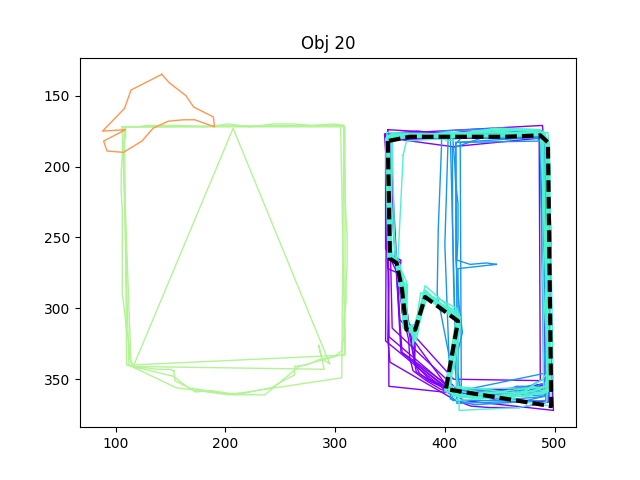
\includegraphics[width=\textwidth]{plots/20.png}
      \caption{Example image showing clustering performed on the same object from Figure \ref{error_examples}.}
      \label{cluster_example}
    \end{figure}
\par Clustering results can also be used as a preprocessing step to any of the quality evaluation algorithms that we discussed earlier. On average, clustering results in ----\% increase in --- across the --NUMBER--- aforementioned algorithms. In particular, we see a greater improvement with clustering preprocessing for algorithms that are not very robust in resolving semantic errors or ambiguity, such as for the \texttt{num pts} retrieval algorithm, than compared to the aggregation-based methods. 
\par Compared to using a metric-based heuristic to detect and eliminate these errors, clustering has additional benefit of preserving worker's semantic intentions in the case where there are multiple instances of different errors. For example, in Figure \ref{cluster_example}, the mistakened clusters included semantic concepts ``monitor'' and ``turtle''. While these are considered bad annotations for this particular task, this cluster of annotation can provide more data for another semantic segmentation task ``monitor''. A potential direction of future work includes adding a additional crowdsourcing task for semantic labelling of clusters (which is cheaper and more accurate than segmentation) to enable reuse of annotations across objects and lower the cost of data collection. 